\documentclass[12pt]{article}
\usepackage[italian]{babel}
\usepackage{natbib}
\usepackage{url}
\usepackage[utf8x]{inputenc}
\usepackage{amsmath}
\usepackage{graphicx}
\graphicspath{{images/}}
\usepackage{parskip}
\usepackage{fancyhdr}
\usepackage{vmargin}
\usepackage{float}
\usepackage{hyperref}
\usepackage{subcaption}
\setmarginsrb{3 cm}{2.5 cm}{3 cm}{2.5 cm}{1 cm}{1.5 cm}{1 cm}{1.5 cm}

\title{HAR Bayesian Network}								% Title
\author{Artifoni Mattia \\ Brena Luca \\ Bottoni Federico}								% Author
\date{Giugno 2019}											% Date

\makeatletter
\let\thetitle\@title
\let\theauthor\@author
\let\thedate\@date
\makeatother

\pagestyle{fancy}
\fancyhf{}
\rhead{Artifoni M. Brena L. Bottoni F.}
\lhead{\thetitle}
\cfoot{\thepage}

\begin{document}

%%%%%%%%%%%%%%%%%%%%%%%%%%%%%%%%%%%%%%%%%%%%%%%%%%%%%%%%%%%%%%%%%%%%%%%%%%%%%%%%%%%%%%%%%

\begin{titlepage}
	\centering
    \vspace*{0.5 cm}
    
\includegraphics[scale = 0.75]{images/LogoBicocca.pdf}\\[1.0 cm]	% University Logo
    \textsc{\LARGE Università degli studi di}\\[0.2 cm]
    \textsc{\LARGE Milano-Bicocca}\\[2.0 cm]	% University Name
	\textsc{\Large F1801Q145}\\[0.5 cm]				% Course Code
	\textsc{\large Modelli probabilistici per le decisioni}\\[0.5 cm]				% Course Name
	\rule{\linewidth}{0.2 mm} \\[0.4 cm]
	{ \huge \bfseries \thetitle}\\
	\rule{\linewidth}{0.2 mm} \\[1.5 cm]

	\begin{minipage}{0.4\textwidth}
		\begin{flushleft} \large
			\emph{Studenti:}\\
			\theauthor
			\end{flushleft}
			\end{minipage}~
			\begin{minipage}{0.4\textwidth}
			\begin{flushright} \large
			\emph{Matricole:} \\
			807466 \\ 808216 \\ 806944
		\end{flushright}
	\end{minipage}\\[2 cm]

	{\large \thedate}\\[2 cm]

	\vfill

\end{titlepage}

%%%%%%%%%%%%%%%%%%%%%%%%%%%%%%%%%%%%%%%%%%%%%%%%%%%%%%%%%%%%%%%%%%%%%%%%%%%%%%%%%%%%%%%%%

\tableofcontents
\pagebreak

%%%%%%%%%%%%%%%%%%%%%%%%%%%%%%%%%%%%%%%%%%%%%%%%%%%%%%%%%%%%%%%%%%%%%%%%%%%%%%%%%%%%%%%%%



\section{Introduzione}
Il progetto ha l'obiettivo di creare un modello di Rete Bayesiana capace di predire il tipo di azione che sta effettuando un ipotetico individuo che indossa il "HAR wearable devices setup", una particolare sistema indossabile composto da 4 accelerometri che permette di analizzare i vettori accelerazione dei sensori in questione. Viene fornito dal progetto di riferimento\cite{HAR} un dataset contenente dati sufficienti per effettuare training e testing del modello

\subsection{Dominio di riferimento}
La semantica dei dati utilizzati è definita nel paper\cite{Paper} del progetto di provenienza. La singola entry del dataset rappresenta uno snapshot acquisito dai sensori e consiste in:
\begin{itemize}
	\item user: username dell'individuo in oggetto (string).
	\item gender: genere del soggetto (string).
	\item age: età dell'individuo (int).
	\item how\_tall\_in\_meters: altezza del soggetto espressa in metri (int).
	\item weight: peso espresso in kilogrammi (int).
	\item body\_mass\_index: indice di massa corporea. Si ottiene dividendo il peso per il quadrato dell'altezza (float).
	\item xi: intero che esprime la componente x del vettore accelerazione nel sensore i-esimo (int).
	\item yi: intero che esprime la componente y del vettore accelerazione nel sensore i-esimo (int).
	\item zi: intero che esprime la componente z del vettore accelerazione nel sensore i-esimo (int).
	\item class: è la variabile target della previsione e indica l'azione eseguita dal soggetto al momento della rilevazione dei dati. Può assumere il valore di "walking", "standing", "standingup", "sitting" e "sittingdown" (string).
\end{itemize}


\subsection{Ipotesi e assunzioni}
Durante lo studio del caso sono state discrimate le features utili al training della rete (i vettori dei sensori) da quelle assunte come superflue (user, gender, age, weight, body\_mass\_index) le quali potrebbero essere utilizzate per specializzarla ulteriormente.\newline
La scelta riguardo all'attributo \emph{how\_tall\_in\_meters} non è stata particolarmente immediata dato che il training set è definito su un range di 13cm (1.58m - 1.71m) che distribuito in un corpo umano non fornisce l'informazione necessaria per poter affermare che tutti i sensori si trovano 13cm più o meno vicini al terreno. La rete dovrebbe essere comunque in grado di predire le azioni di un bambino, il quale ha altezza decisamente inferiore rispetto a quella precedentemente descritta, ciò nonostante assumiamo che l'altezza dell'utente ricada all'interno del range descritto dato che in alcuni test affrontati, la complessità della rete era tale da scatenare MemoryError nella rappresentazione dei dati.

\section{Scelte di design}
\subsection{Analisi statistica e qualitativa}
\begin{figure}[H]
	\centering
	{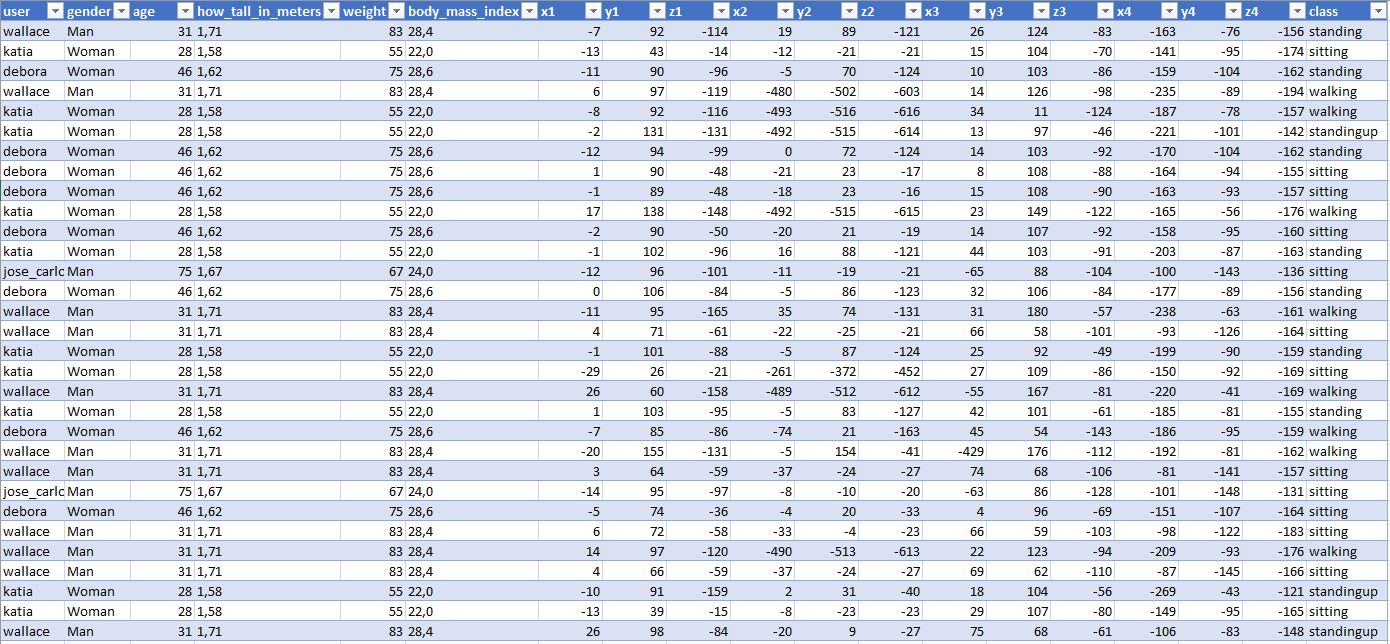
\includegraphics[width=1\textwidth]{images/dataset.JPG}}
	\caption{Dataset dopo lo shuffle}
	\label{fig:dataset}
\end{figure}
Il dataset si presenta come in figura \ref{fig:dataset} dopo una prima fase di pulizia, in cui sono stati individuati e puliti alcuni caratteri non necessari tra i campi e timestamp inaspettati tra le entry della tabella, ed una seconda di shuffle, nella quale i record sono stati randomizzati. \newline
E' stata effettuata inoltre una fase di analisi statistico-descrittiva considerando le features che assumono valori in range indefiniti per cercare di individuare qualche distribuzione particolare o comportamento anomalo. Osservando le misurazioni di media e deviazione standard tra le variabili, si è notato che per alcune di esse i valori assunti di massimo e di minimo risultavano particolarmente distanti dal valor medio. Si è deciso pertanto di individuare e contare i record contenenti tali valori. Rappresentando una minoranza non significativa per la successiva fase di modellazione della rete, si è deciso pertanto di rimuoverli.


\begin{table}[h]
	\caption{Analisi descrittiva del dataset}\label{tab:analytics}
	\begin{tabular}{|l|l|l|l|l|l|}
		\hline
		Campo & Min & Max & Media & Moda & DevStd \\
		\hline
		x1 & -306 & 509 & -6.649327127 & -1 & 11.61623803 \\
		y1 & -271 & 533 & 88.29366732 & 95 & 23.89582898 \\
		z1 & -603 & 411 & -93.16461092 & -98 & 39.40942342 \\
		x2 & -494 & 473 & -87.82750418 & -492 & 169.4351938 \\
		y2 & -517 & 295 & -52.06504742 & -516 & 205.1597632 \\
		z2 & -617 & 122 & -175.0552004 & -616 & 192.8166147 \\
		x3 & -499 & 507 & 17.42351464 & 38 & 52.63538753 \\
		y3 & -506 & 517 & 104.5171675 & 108 & 54.15584251 \\
		z3 & -613 & 410 & -93.88172647 & -102 & 45.38964613 \\
		x4 & -702 & -13 & -167.6414483 & -164 & 38.31134199 \\
		y4 & -526 & 86 & -92.62517131 & -94 & 19.96861022 \\
		z4 & -537 & -43 & 88.29366732 & -162 & 13.22102006 \\
		
		\hline
	\end{tabular}
\end{table}

Dalla tabella \ref{tab:analytics} si può notare che i range di variabilità degli attributi non seguono comportamenti particolari, tanto meno le distribuzioni che in alcuni casi sono caratterizzati da deviazione standard particolarmente bassa (come il caso di \emph{x1}) mentre in altri casi molto alta (come \emph{y2}).


\begin{figure}[h]	
	\begin{subfigure}{0.5\textwidth}
		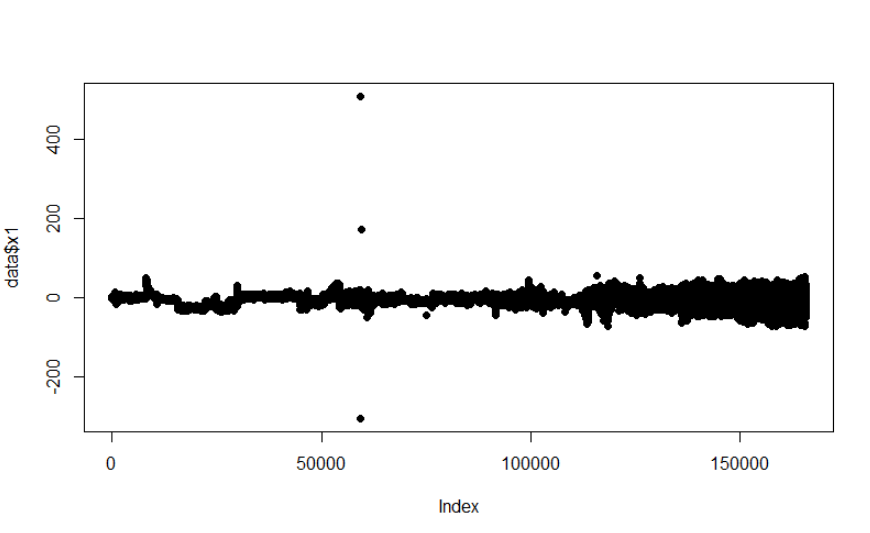
\includegraphics[width=0.9\linewidth, height=5cm]{images/x1notnormalize.PNG} 
		\caption{x1 non normalizzata.}
		\label{fig:x1nonNormalize}
	\end{subfigure}
	\begin{subfigure}{0.5\textwidth}
		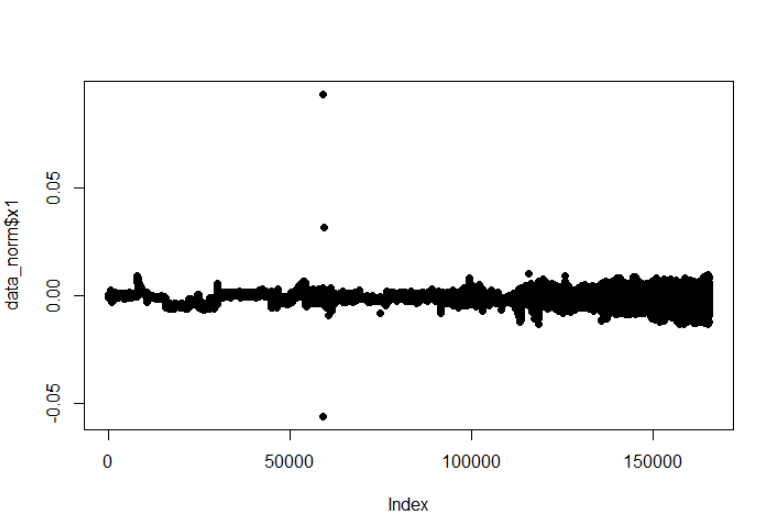
\includegraphics[width=0.9\linewidth, height=5cm]{images/x1normalize.PNG}
		\caption{x1 normalizzata.}
		\label{fig:subim2}
	\end{subfigure}
	\begin{subfigure}{0.5\textwidth}
		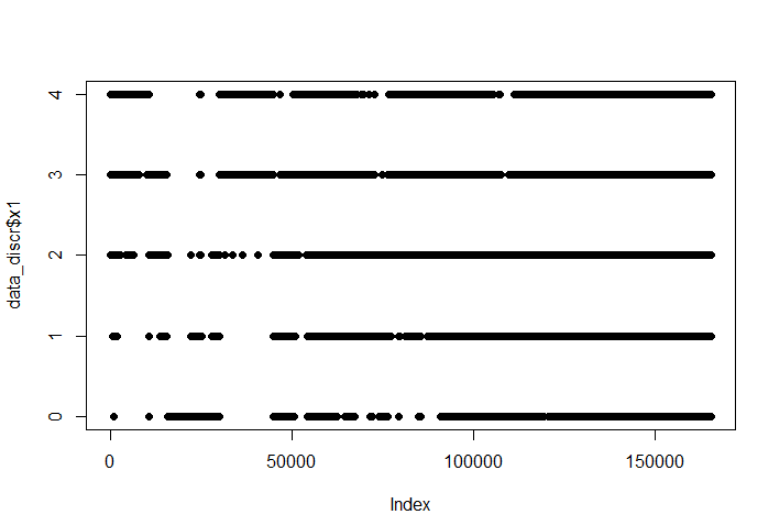
\includegraphics[width=0.9\linewidth, height=5cm]{images/x1discretize.PNG}
		\caption{x1 normalizzata e discretizzata.}
		\label{fig:subim3}
	\end{subfigure}
	\caption{Normalizzazione e discretizzazione della feature x1.}
	\label{x1}
\end{figure}

\subsection{Normalizzazione}
Nella fase embrionale della progettazione la normalizzazione era stata ignorata. Infatti la predizione lavorava su features che avevano range piuttosto incosistenti al variare del sensore e della componente del vettore accelerazione considerata. Questo si può notare dalle colonne \textit{Min} e \textit{Max} in tabella \ref{tab:analytics}, che si riferisce ai dati grezzi parzialmente ripuliti. Quindi si è pensato di effettuare una normalizzazione per ogni feature, in modo da compattare i valori tra -1 e 1 andando anche a eliminare gli outliers. \par
Di seguito, nelle figure \ref{x1} e \ref{z4}, sono presentati alcuni grafici che illustrano la distribuzione dei valori di alcune features prima e dopo la normalizzazione. A seguito dell'operazione di normalizzazione il dataset appare come riportato in figura \ref{normalized}.

\begin{figure}[H]
	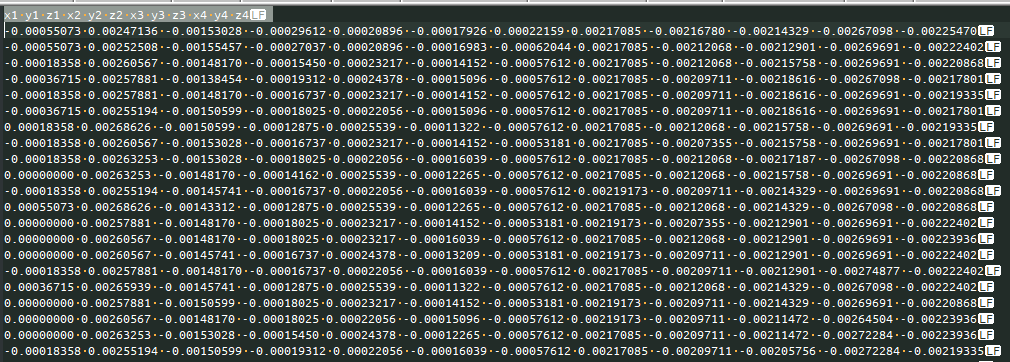
\includegraphics[width=1\textwidth]{images/datasetNormalizzato.PNG}
	\caption{Il dataset normalizzato.}
	\label{normalized}
\end{figure}


\begin{figure}[h]
	
	\begin{subfigure}{0.5\textwidth}
		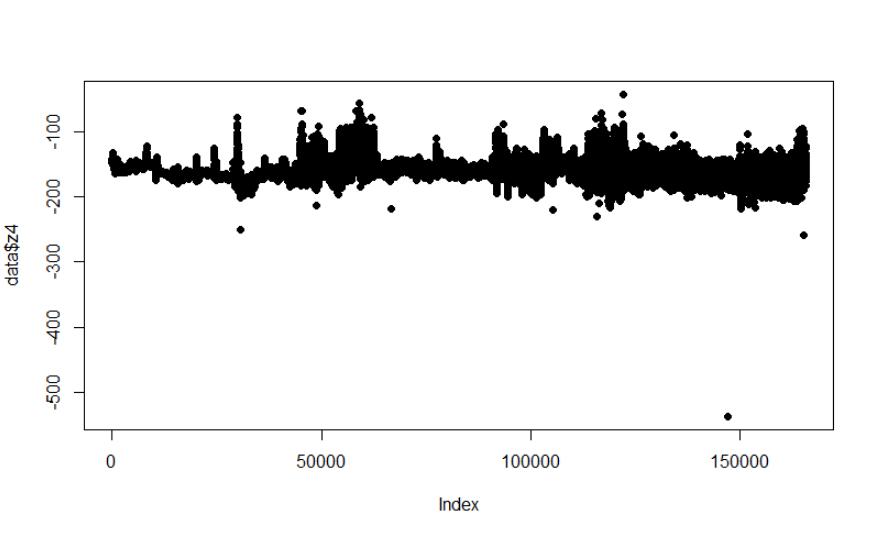
\includegraphics[width=0.9\linewidth, height=5cm]{images/z4notnormalize.PNG} 
		\caption{z4 non normalizzata.}
		\label{x1nonNormalize}
	\end{subfigure}
	\begin{subfigure}{0.5\textwidth}
		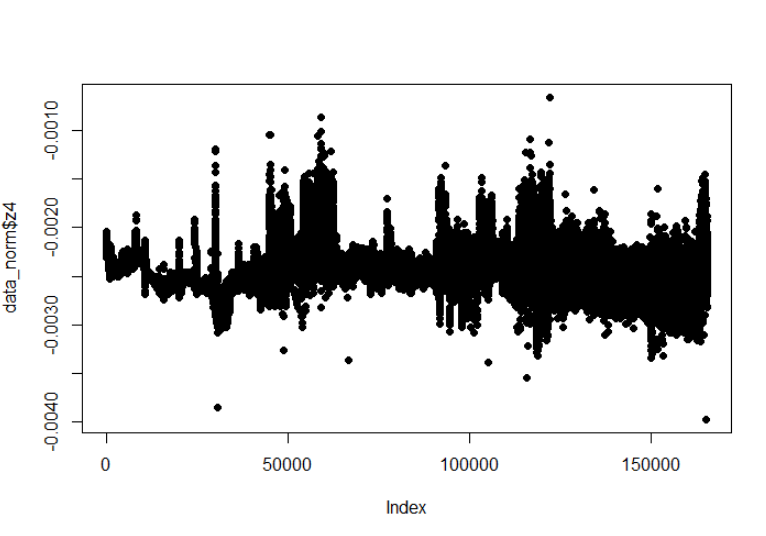
\includegraphics[width=0.9\linewidth, height=5cm]{images/z4normalize.PNG}
		\caption{z4 normalizzata.}
		\label{subim2}
	\end{subfigure}
	\begin{subfigure}{0.5\textwidth}
		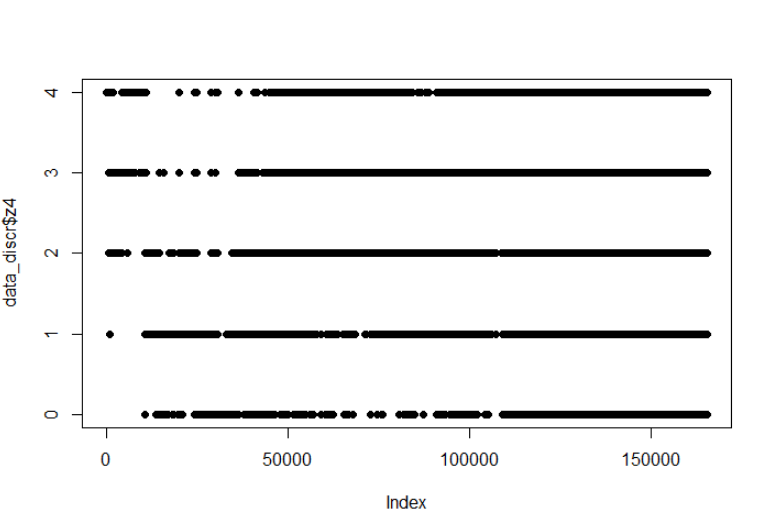
\includegraphics[width=0.9\linewidth, height=5cm]{images/z4discretize.PNG}
		\caption{z4 normalizzata e discretizzata.}
		\label{subim2}
	\end{subfigure}
	\caption{Normalizzazione e discretizzazione della feature x1.}
	\label{z4}
\end{figure}

\subsection{Discretizzazione}
I valori delle features nel dataset originale sono continui. Per lavorare con le reti Bayesiane, fornite dalle librerie \cite{scikit-learn} e \cite{pomegranate} (che non implementano la gestione di variabili continue), è stato necessario ricorrere alla discretizzazione dei dati.\par
Inizialmente i dati sono stati suddivisi in partizioni a range identici senza tenere conto di come questi fossero distribuiti. Successivamente abbiamo realizzato come questa procedura fosse imprecisa dopo aver osservato il modo in cui le distribuzioni di probabilità si sbilanciavano prevalentemente verso una sola classe della variabile. \newline
La discretizzazione definitiva è stata applicata sul dataset normalizzato. Per discretizzare i dati sono stati scelti 5 intervalli o bins. La funzione scelta (KBinsDiscretizer della libreria sklearn \cite{scikit-learn}) adatta automaticamente il numero dei bins in modo che la distribuzione dei dati in essi sia omogenea. Uno sapshot dei dati discretizzati è raffigurato nell'immagine \ref{fig:discretized}

\begin{figure}[h]
	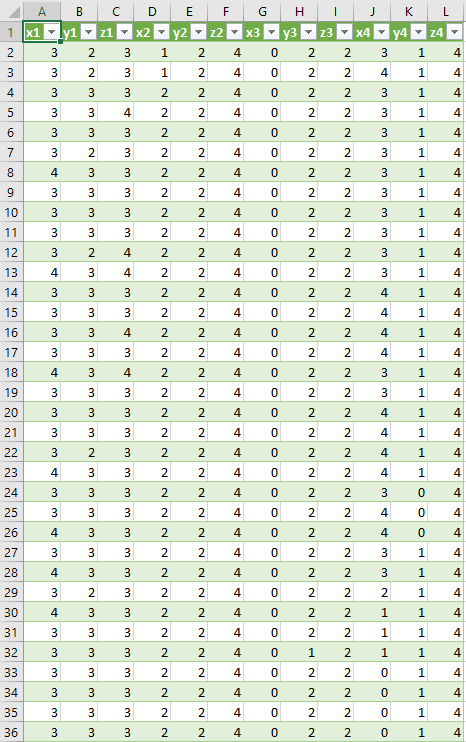
\includegraphics[scale = 0.5]{images/datasetDiscretizzato.PNG}
	\caption{Il dataset discretizzato.}
	\label{fig:discretized}
\end{figure}


\section{I modelli di rete}
\subsection{pgmpy}
Il software inizialmente scelto è pgmpy\cite{pgmpy} di Python, una libreria che permette di modellare le dipendenze in modo agile e stimare le CPT delle variabili sfruttando dei metodi che accettano il dataset ed infine effettuare inferenze dichiarando la variabile di query e le evidenze. \linebreak
Utilizzando la libreria ci siamo resi conto di come sia performante utilizzando modelli semplici e correlati da pochi record, tuttavia appena è avvenuta l'esecuzione della stima delle CPT nel primo modello completo ideato abbiamo riscontrato le prime difficoltà.

\subsubsection{Modello correlato}
L'idea che sta alla base di questo primo modello consiste nello stimare le dipendenze tramite lo strumento statistico \emph{indice di correlazione di Paerson}, assumendo che se due feautres hanno distribuzioni simili (e quindi alta correlazione diretta o inversa) allora vi è una dipendenza tra le due. Sono state così selezionate le relazioni scartando le simmetrie e stimate le CPT tramite il metodo \emph{MaximumLikelihoodEstimator} della libreria basandosi sui sample passati come parametro. \newline

\begin{figure}[H]
	\centering
	{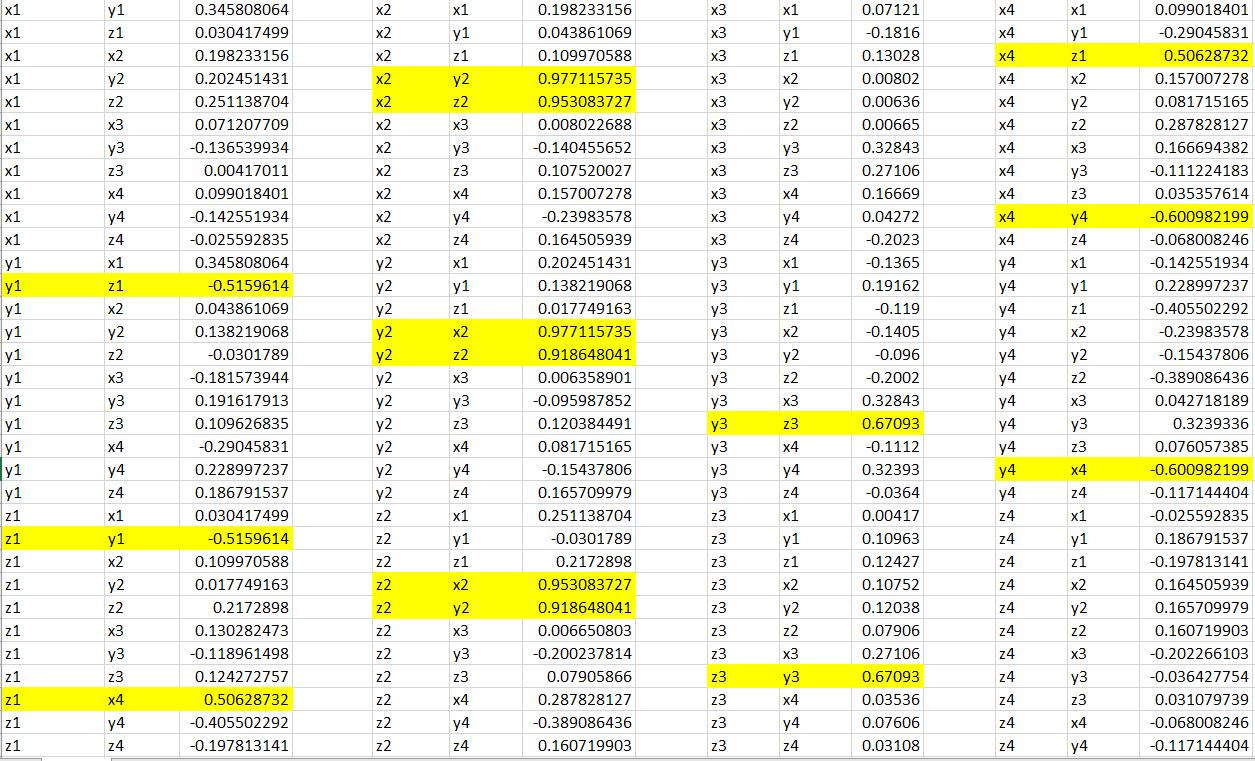
\includegraphics[width=1\textwidth]{images/corr05.JPG}}
	\caption{Indice di correlazione di Paerson calcolato su tutte le le combinazioni di componenti}
	\label{fig:corr}
\end{figure}

Successivamente abbiamo stimato la precisione del modello calcolando il rapporto tra le inferenze corrette su quelle totali. Il metodo utilizzato, \emph{query}, si occupa di effettuare la singola previsione. Abbiamo notato che a parità di modello, raddoppiando il numero delle classi per ogni variabile, il tempo impiegato dalla funzione aumenta vertiginosamente, perciò abbiamo stimato la precisione del modello più complesso possibile ma con tempi di esecuzione nella norma. \newline
Il modello consiste in cinque classi per ogni variabile e le seguenti dipendenze tra le variabili:\newline \emph{[('x1', 'class'),('x3', 'class'),('y4', 'class'), ('z1', 'class'), ('z2', 'class'), ('z3', 'class'), ('z4', 'class'), ('y1', 'z1'), ('x2', 'y2'), ('x2', 'z2'), ('y2', 'z2'), ('y3', 'z3'), ('x4', 'z1'),  ('x4', 'y4')]}.\newline
La precisione stimata è del 54\%, un valore troppo basso per giustificare la computazione così lunga e dispendiosa di risorse. Abbiamo deciso così di tentare con un modello differente.

\subsubsection{Generazione del modello}
Dato l'insuccesso del modello correlato abbiamo cercato di generare la miglior configurazione di dipendenze secondo la libreria. Dopo il lancio della funzione che si occupa di chiamare l'API per la generazione abbiamo atteso circa 8 ore e successivamente interrotto l'esecuzione. Forse per la mole di dati, forse per la discretizzazione del dataset o forse per la natura stessa dell'algoritmo, non vi è stato alcun risultato.

\subsection{pomegranate}
Alla luce dei test effettuati abbiamo deciso di utilizzare un'altra libreria: Pomegranate \cite{pomegranate}, secondo gli utenti di alcuni forum, dovrebbe essere performante anche nei casi in cui \emph{pgmpy} non lo è. La libreria è nota inoltre per avere API molto simili a quelle di scikit-learn \cite{scikit-learn} (uno tra i software leader nel campo del Machine Learning) 

\subsubsection{Modello generato}
Il modello proposto viene generato automaticamente dalla libreria tramite la funzione \emph{from\_samples} la quale genera gli stati della rete e le dipendenze basandosi sul training-set passato, dando all'utente la possibilità di esportare un file JSON (poco comprensibile) contente tutti i dati del modello. Oltre a questa non vi sono altre API per ottenere informazioni riguardo alla rete.\newline
Nonostante la lunga attesa per poter ottenere i dati riguardo all'accuratezza del modello, i risultati sono più che soddisfacenti \ref{tab:results}, tra cui Accuracy del modello: 97\%.\newline
\begin{table}[h]
	\caption{Score del modello}\label{tab:results}
	\begin{tabular}{|l|l|l|l|}
		\hline
		Campo & Precision & Recall & F1 Score\\
		\hline
		Walking & 97\% & 97\% & 97\% \\
		Standing & 99\% & 98\% & 98\% \\
		Standingup & 90\% & 87\% & 90\% \\
		Sitting & 99\% & 99\% & 99\% \\
		Sittingdown & 86\% & 92\% & 89\% \\
		\hline
	\end{tabular}
\end{table}
Un fatto che ci ha particolarmente colpito del modello generato da Pomegranate è che in alcuni casi le inferenze venivano restituite dall'API senza essere state risolte. Ipotizziamo che quando la rete non è in grado di effettuare una decisione, restituisce \emph{None} invece di assegnare una valore casuale al risultato. Queste particolari inferenze sono state ignorate nel calcolo delle performance dato che il numero di esse è estremamente ridotto, circa lo 0.09\% delle totali. \newline
Date le notevoli performance del modello, è stato sviluppato un software che permette di istanziare il modello e lanciare una o più inferenze, eseguibile tramite '\emph{python inference.py "x1=-5;y1=30;z1=-20;x2=..."}' e viene restituito in output la predizione. Nel caso il parametro stringa venga omesso, il software elabora un array di stringhe in "inference/in.txt", le interpreta come query alla variabile \emph{class} del modello e stampa in "inference/out.txt" i risultati. 
\clearpage
\section{Conclusioni}

L'obiettivo di questo lavoro è inferire l'azione compiuta da un soggetto tramite i dati rilevati da un sistema di 4 accelerometri. La previsione è stata ottenuta mediante una rete Bayesiana che modella le dipendenze tra i sensori, visti come variabili casuali.\par L'obiettivo è stato raggiunto tramite l'approccio \textit{learning structure by data,} dopo aver provato inizialmente a individuare la struttura tramite uno studio di correlazione manuale tra i dati. Il modello generato riesce a inferire l'azione compiuta dal soggetto con una precisione molto alta, di circa 97\%. Inoltre, i sample del dataset sono ben distribuiti tra le varie attività, quindi quando il modello viene generato, la fase di shuffle e di campionamento dei sample non influiscono sulla precisione nell'inferenza. Una difficoltà importante riportata nella progettazione è la mancata visualizzazione della struttura della rete. Infatti i risultati riportati sono stati ottenuti con la libreria \cite{pomegranate} che si è scoperto essere sprovvista delle API per la visualizzazione dello scheletro e in generale poco documentata e supportata. L'unica funzione disponibile è l'esportazione tramite JSON che pero' risulta in un file difficilmente interpretabile.\newline
Un altro fattore inaspettato che ci ha colpito negativamente sono i tempi di esecuzione delle due librerie utilizzate che, nonostante Pomegranate sia notevolmente più ottimizzato di Pgmpy, sono decisamente alti.

\newpage
\bibliographystyle{plain}
\bibliography{biblist}

\end{document}
